% PKUMpLtX --- A LaTeX document class for 'Modern Physics Laboratory' in PKU based on `revtex4-2`
%
% Please read `README.md' and the template file before using
% 需要确保 font 选项指定的字体已安装! 具体参见 `README.md' 的说明.
\documentclass[font=fandol]{mpltx}

% 以下至 \begin{document} 都仅是本文件为了方便额外定义的命令, 写报告时不需要.
\hypersetup{colorlinks=true}% 超链接带颜色
\usepackage{xcolor}
\usepackage{tcolorbox}

\newtcbox{\buttombox}[1][red]
  {on line, arc = 3pt, outer arc = 3pt,
    colback = #1!10!white, colframe = #1!50!black,
    boxsep = 0pt, left = 2pt, right = 2pt, top = 1pt, bottom = 1pt,
    boxrule = 1pt}

\newcommand{\note}[1]{{\color{gray}#1}}
\NewDocumentCommand{\pkg}{s o m}{%
    \IfBooleanF{#1}{%
        \IfNoValueTF{#2}%
            {\href{https://www.ctan.org/pkg/#3}}%
            {\href{https://www.ctan.org/pkg/#2}}%
    }%
    {\textsf{#3}}%
}
\newcommand*\cs[1]{\texttt{\textbackslash #1}}
\newcommand*\env[1]{\textit{\texttt{#1}}}
\newcommand*\code[1]{\texttt{#1}}
\newcommand*\file[1]{\textbf{\texttt{#1}}}
\makeatletter
\newcommand\releasedate{%
    \href{https://github.com/CastleStar14654/PKUMpLtX/releases/tag/\mpltx@fileversion}%
        {\mpltx@filedate, \mpltx@fileversion}}
\makeatother
% 以上是本文件为了方便额外定义的命令, 写报告时不需要.

\begin{document}

\title{体效应振荡器的工作特性和波导管的工作状态} % 切合报告内容, 简短明确, 可以不同于讲义
\author{罗俊熙} % 这里 \emailphone 一定要紧跟在 \author 后方
\emailphone{see.looooo@stu.pku.edu.cn}{(86)13611162432}
% 如果改用 \email 则仅需要邮箱参数
\affiliation{北京大学物理学院\quad 学号: 2000012508}
% % 可以使用 \zhdate 自动生成中文日期, 如
% \date{\zhdate{2020/12/1}}
% % 也可使用 babel 的 \localedate, 如
% \date{\localedate{2020}{12}{1}}
% % 两者均会输出 `2020 年 12 月 1 日'
% 下面的 \date 的参数是为了自动输出正确版本号, 正式报告请替换为上面的两种 \date 之一
\date{\localedate{2023}{03}{02}}
\begin{abstract}
	微波是一种被广泛应用的电磁波,产生微波的方法有很多,而这次实验将通过体效应振荡器,产生微波,并测量其工作特性;然后测量微波在波导管中的波导波长,传输特性等,进而推算出光速和验波律等性质。
\end{abstract}
\keywords{微波, 波导管, 体效应振荡器}

\maketitle

\section{引言}
微波是一种波长很短,频率很高的电磁波,其性质让其很好地应用在国防、通讯和农业生产上,为了了解微波的产生和传输特性,掌握有关微波的基本参量,如功率、频率、电压和驻波比等的测量原理和方法是必不可少的。
微波通常由一些特殊的电子管如速调管和磁控管等产生,而实验中常使用体效应振荡器和雪崩振荡器等来产生微波。这次实验就使用了体效应振荡器产生的微波源。
微波能在波导管中传播,分为三种状态:匹配状态、驻波状态和混波状态,而其在波导中传播的相速度大于光速,可以通过测量频率和波导波长的方法来确定相速度、群速和和光速。
本次实验主要是了解体效应振荡器的一些性质,并掌握微波三种基本参量的测量方法,确定波导波长和波导管中的传播速度。

\section{理论}\label{sec:theory}
\subsection{体效应振荡器}
体效应振荡器主要通过Gunn效应,在n型的砷化锭单晶上产生很高的电流振荡,然后辐射出微波。这个效应的成因是因为这种材料具有负的微分迁移率的区域,令内部产生“高场畴”,当高场畴传播到导体边界时,就会产生电流脉冲,进而转化为微波。
这种脉冲是周期性的,其频率为:
$$f=\frac{1}{T_D}=\frac{v_d}{L}$$
式中,$T_D$是畴的渡越时间,而$L$为样品的长度,$v_d$为畴的运动速度。
\subsection{体效应振荡器的工作特性}
将体效应二极管放在高$Q$的谐振腔中,构成电路,就能产微波振汤,而本次实验使用的固态源则是使用机械调谐的方式,产生特定频率的微波。机器内部具有一个非接触活塞,可以改变谐振腔的有效长度,改变振荡频率,活塞移入腔内越多,电容减少,工作频率提升。因为每个体效应二极管的掺杂、缺陷或位错等都不一样,因此其工作电压、频率等关系都不一样。
\subsection{波导管中波的传播特性}
波导管中能通过特定波长的电磁波,由于麦克斯韦方程式的限制,电磁场在其内部只能以特定的模式传播,这次实验的方形波导管,就只能通过$\rm{TE_1}$的模式,其特色是在导管中形成垂直波导寛壁的电场,而且传播的波导波长和自由空间并不一样。满足:
$$c=\lambda f, \quad v_g=\lambda_gf$$
其中$c$为光速,$v_g$为相速度。而理论表明,光在其内的相速度是大于光速的。因此我们可以通过测定波导波长$\lambda_g$和频率$f$来找出光速$c$。
\subsection{驻波测量}
我们可以通过驻波测量线来进行驻波比和波导波长的测量,将系统调节至匹配的状态,而驻波比则是如下定义的
$$\rho=\frac{|E_{\max}|}{|E_{\min}|}$$
其中$E$为驻波线测得的场强。调节的方法则是通过单螺螺调配器和驻波测量线的交互调节,来形成不同的驻波比,,驻波比反射率有着以下关系:
$$\Gamma_0=\frac{\rho -1}{\rho+1}$$
这次实验的后半部分,需要在驻波的状态下进行。
\subsection{检波特性曲线和检波律}
在测量驻波比时,检波晶体会有辅出信号测出,晶体的检波电流$I$和传输线探针周围的电场$E$满足:
$$I=k_1E^n$$
其中$k_1$和$n$都是一些常数,一般地$n$都很接近$2$,称为平方律检波。进行测量时,会先将测量线终端短路,驻波振幅与终端距离满足的关系为:
$$|E|=k_2|\sin{(\frac{2\pi l}{\lambda_g})}|$$
我们可以通过检波电流关于$l$的曲线$I(l)$和$E$来求得常数$n$进而得到晶体的检波律,一般地,我们可以用下列关系式定出$n$:
$$n=\frac{-0.3010}{\log_{10}{\cos{(\frac{{\pi\Delta l}}{\lambda_g})}}}$$
其中$\Delta l$为驻波曲线上$I=I_m/2$两点距离。

\section{实验装置}
本次实验使用的微波信号由DH1121A型\qty{3}{\cm}固态信号源提供,而主要元件有隔离器、衰减器、吸引式频率计、驻波测量线和单螺调配器。如\autoref{fig:0}搭建线路,其中A和B都是电流表,用以示波作用。
\begin{figure}
	\centering
	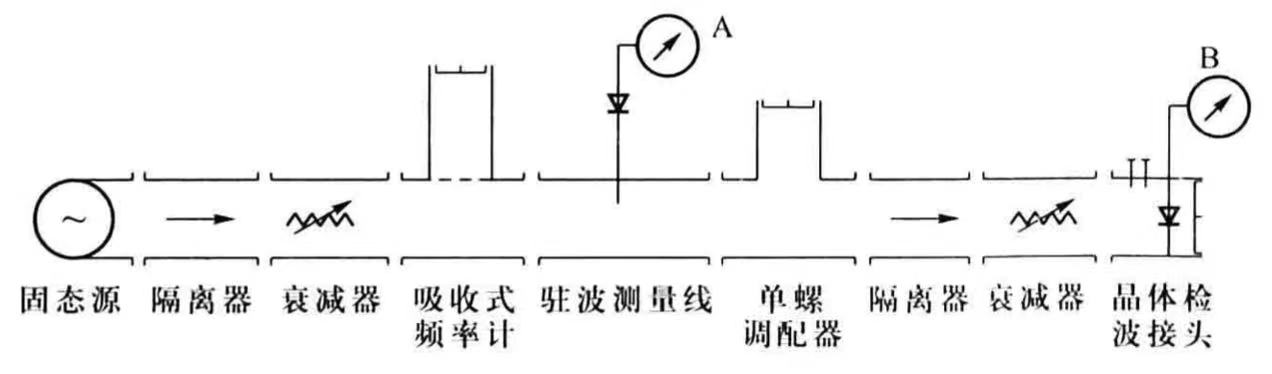
\includegraphics[width=0.85\linewidth]{fig/0.jpg}
	\caption{实验线路图\cite{jindaishiyan}}
	\label{fig:0}
\end{figure}

\section{实验内容}
\begin{enumerate}
	\item 测量体效应振荡器的工作电压与工作电流、输出功率及频率的特性曲线;
	\item 测量振荡频率和输出功率的关系曲线;
	\item 调节和测量小驻波比和中驻波比的线路,并计算其反射率$\Gamma_0$;
	\item 测量波导波长、光速、相速度和群速度;
	\item 测量驻波曲线和计算出检波律常数$n$。
\end{enumerate}

\section{实验过程、结果及讨论}
\subsection{观测体效应振荡器的工作特性}
将信号源置于\buttombox[blue]{等幅}状态,调节\buttombox[blue]{频率},使其至$\qty{9.000}{\GHz}$,预热$\qty{30}{\minute}$。
\par
按下\buttombox[blue]{教学},通过\buttombox[blue]{电压}按钮,在$0\sim\qty{13.0}{\V}$连续改变工作电压,得到频率计和光点检流计B,测得微波频率和相对功率(注要调节短路活塞和单螺调配器),使检波接头输出最大。实验结果\autoref{fig:1},可以看出,在低压时体效应管的工作电流和工作电压成正比,随着电压增大,工作电流会出现一个高峰,稍稍下降后,在\qty{7.5}{\V}出现饱和。而输出的微波频率会随着电压增大而慢慢降低。而输出相对功率则在工作电流饱和后,慢慢增大,大致呈现线性关系。

\begin{figure}
	\centering
	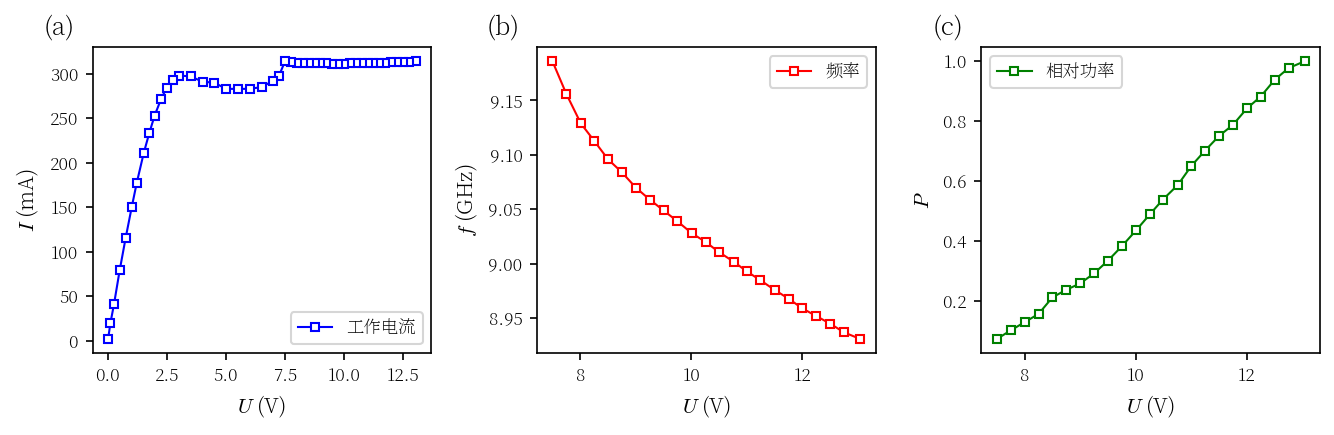
\includegraphics[width=0.85\linewidth]{fig/1.png}
	\caption{体效应振荡器工作电压和微波输出关系图。(a):工作电压与工作电流关系;(b):工作电压与输出频率关系;(c):工作电压与相对功率关系}
	\label{fig:1}
\end{figure}



\subsection{改变谐振腔的有效长度,测量振荡频率和输出功率的关系曲线}
提起\buttombox[blue]{教学},使其工作在标准电压$\qty{12.0}{\V}$,此时的工作电流约为$\qty{250}{\mA}$,转动\buttombox[blue]{频率},改变谐振腔尺寸,从而改变其微波频率,然后用频率计做频率测量,得到\autoref{fig:2},从图可以看出,转出相对功率和频率大致成正比。

\begin{figure}
	\centering
	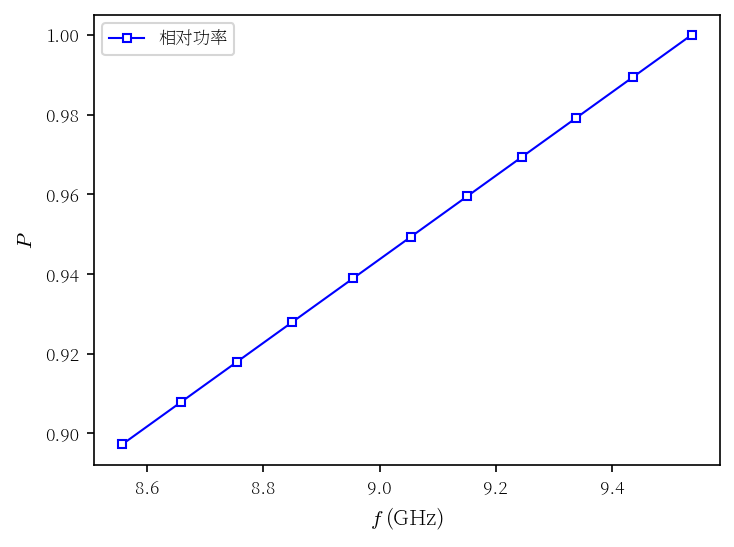
\includegraphics[width=0.85\linewidth]{fig/2.png}
	\caption{输出频率和输出相对功率关系图。}
	\label{fig:2}
\end{figure}


\subsection{练习测量小驻波比和中驻波比}
在\buttombox[blue]{等幅}状态下,使频率显示为$\qty{9.000}{\GHz}$,电压为$\qty{12.0}{\V}$,调整好驻波测量线,利用单螺调配器改变测量线的终端状态,调节到匹配状态,测量小驻波比,如\autoref{tab:1}

\begin{table}
	\caption{相对功率与驻波比和反射率关系}
	\label{tab:1}
	\begin{ruledtabular}% ruledtabular 环境自动生成首尾双横线, 并调整宽度至占满全行
		\begin{tabular}{ccccc}
			序号 & $E_{\max}$ & $E_{\min}$ & $\rho$ & $\Gamma_0$ \\
			\colrule
			1    & 101.0      & 97.9       & 1.032  & $1.57\%$   \\
			2    & 101.6      & 98.0       & 1.036  & $1.77\%$   \\
			3    & 102.5      & 99.0       & 1.035  & $1.72\%$
		\end{tabular}
	\end{ruledtabular}
\end{table}

可以求出,这是的小驻波比为$\bar\rho=1.034$,反射率$\Gamma_0=1.69\%$。

\subsection{测量波导波长和驻波曲线}
调节单螺调配器,使驻波测量线终端接近全反射(即$\rho$值较大),利用平均值法测量极小点两侧的等强点$x_1',x_1''$,
用平均值的方式求得$x'_{\min}=\frac{1}{2}(x_1'+x_1'')$,这里则用三个波节作线性拟合:$x_n=\frac{\lambda_g}{2}\times n + c$,得到\autoref{tab:2},经过线性拟合后,可以得到波导波长:

\begin{table}
	\caption{节点位置测量表}
	\label{tab:2}
	\begin{ruledtabular}% ruledtabular 环境自动生成首尾双横线, 并调整宽度至占满全行
		\begin{tabular}{cccc}
			序号$n$ & $x'$  & $x''$ & $\bar x$ \\
			\colrule
			1       & 89.5  & 90.9  & 90.2     \\
			2       & 113.9 & 115.5 & 114.7    \\
			3       & 138.8 & 140.1 & 139.45
		\end{tabular}
	\end{ruledtabular}
\end{table}

$$\lambda_g=\qty{49.20}{(\mm)}$$

\subsection{测量驻波曲线和$I-|E|$曲线}
在两个波节间,测量出不同位置的相对功率$P$,也即是检波电流$I$,可以得到\autoref{fig:3}(a)的图像,半高位置为$l_1=\qty{88.7}{\mm}$和$l_2=\qty{100.9}{\mm}$,半高宽为$\Delta l = \qty{12.2}{\mm}$,代入公式后计算得到:
$$n=\frac{-0.3010}{\lg{\cos{\frac{\pi\Delta l}{\lambda_g}}}}= 2.037$$
我们也可以通过$|E|$和相对位置$l$的关系$|E|\propto \sin{\frac{2\pi l}{\lambda_g}}$,画出$I-E$曲线,如\autoref{fig:3}(b)所示,并且通过拟合的方式得到检波律:
$$n=1..972$$

计算出自由空间的波长为(导管长边取为$a=\qty{22.86}{\mm}$):
$$\lambda=\frac{\lambda_g}{\sqrt{1+(\frac{\lambda_g}{2a})^2}}=\qty{33.49}{\mm}$$
微波频率测得为$f=\qty{8.953}\GHz{}$,可以得到光速$c$、微波相速度$v_g$和微波群速度$u$为:
$$
\begin{aligned}
	c &=\lambda f = \qty{2.998}{\km\per\s}\\
	v_g &= \lambda_g f=\qty{4.405}{\km\per\s}\\
	u &= \frac{c^2}{v_g}=\qty{2.041}{\km\per\s}
\end{aligned}
$$
可以看出微波在波导中的传播相速度比光速要大,而群速度,则比光速要小。

\begin{figure}
	\centering
	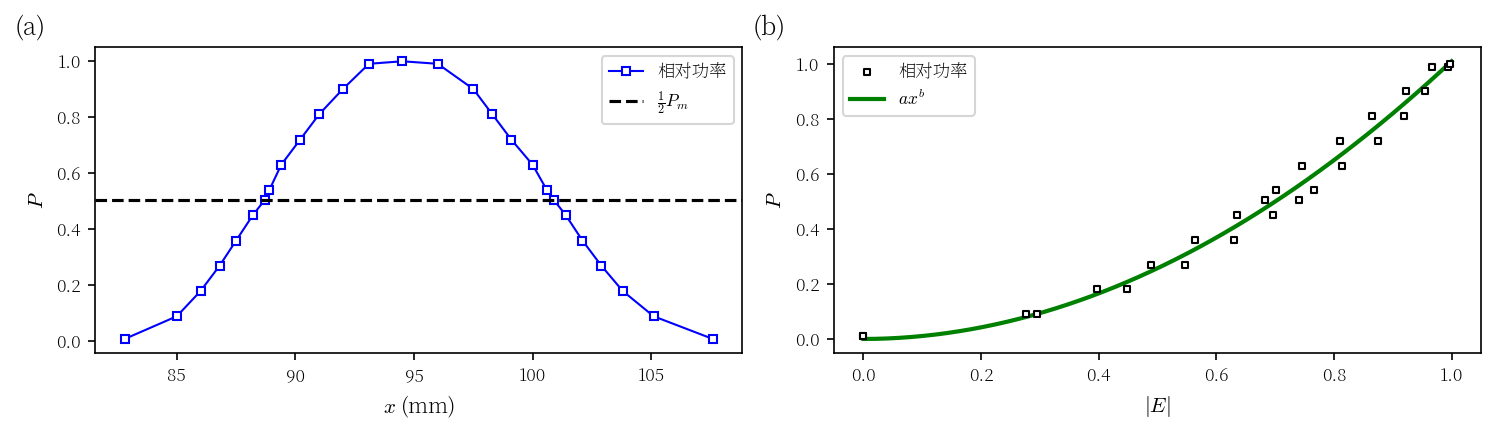
\includegraphics[width=0.85\linewidth]{fig/3.png}
	\caption{(a):位置和相对功率的关系图,两边为波节位置;(b):场强和相对功率的关系图,其中绿色为拟合曲线}
	\label{fig:3}
\end{figure}

\section{结论}
\textbf{经过这次实验,可以得到波导管的工作特性,并且测量出微波在导管中的波导波长、相速度和群速度,并对光速进行了检证,}

\begin{acknowledgments}
	感谢王常生老师的贴心教导。
\end{acknowledgments}

% bibliography 的参数是你的 *.bib 文件去掉后缀名后的部分
\bibliography{bibli}

\clearpage % 附录前另起一页
\appendix % 附录开始
\section{思考题}\label{app:exercise}
\subsection{在$a=\qty{23.0}{\mm}$、$b=\qty{10.0}{\mm}$的矩阵波导管中能不能传播$\lambda=\qty{2}{\cm}$、$\qty{3.0}{\cm}$和$\qty{5.0}{\cm}$的微波?各能传播哪些波型?}

根据$\lambda_c=\frac{2}{\sqrt{(\frac{m}{a})^2+(\frac{n}{b})^2}}$,我们可以得到
$\lambda_{c,10}=\qty{46.0}{\mm}$、$\lambda_{c,01} = \qty{20.0}{\mm}$、$\lambda_{c,11} = \qty{18.3}{\mm}$ 和 $\lambda_{c,20} = \qty{23}{\mm}$。
而波导管能够通频的条件为$\lambda_c>\lambda$,即$\qty{5.0}{\cm}$的波长不能通过,而$\qty{3.0}{\cm}$的波长能以$\rm{TE_{10}}$的模式传播。
而对于波长为$\qty{2}{\cm}$的微波,能以$\rm{TE_{10}}$和$\rm{TE_{20}}$的模式。

\end{document}
